\section{Secure Distance Measurement}

\paragraph{Applications:}
\begin{itemize}
    \item Mitigate car key relay attack.
    \item Mitigate Contact Tracing Wormhole attacks.
    \item Mitigate Car distance spoofing attack.
    \item[-->] We need ranging that is (provably) secure from all logical and physical layer attacks.
\end{itemize}
\vspace{0.2cm}
\textbf{Ranging Techniques}\\
\begin{minipage}{\linewidth}
    \centering      
    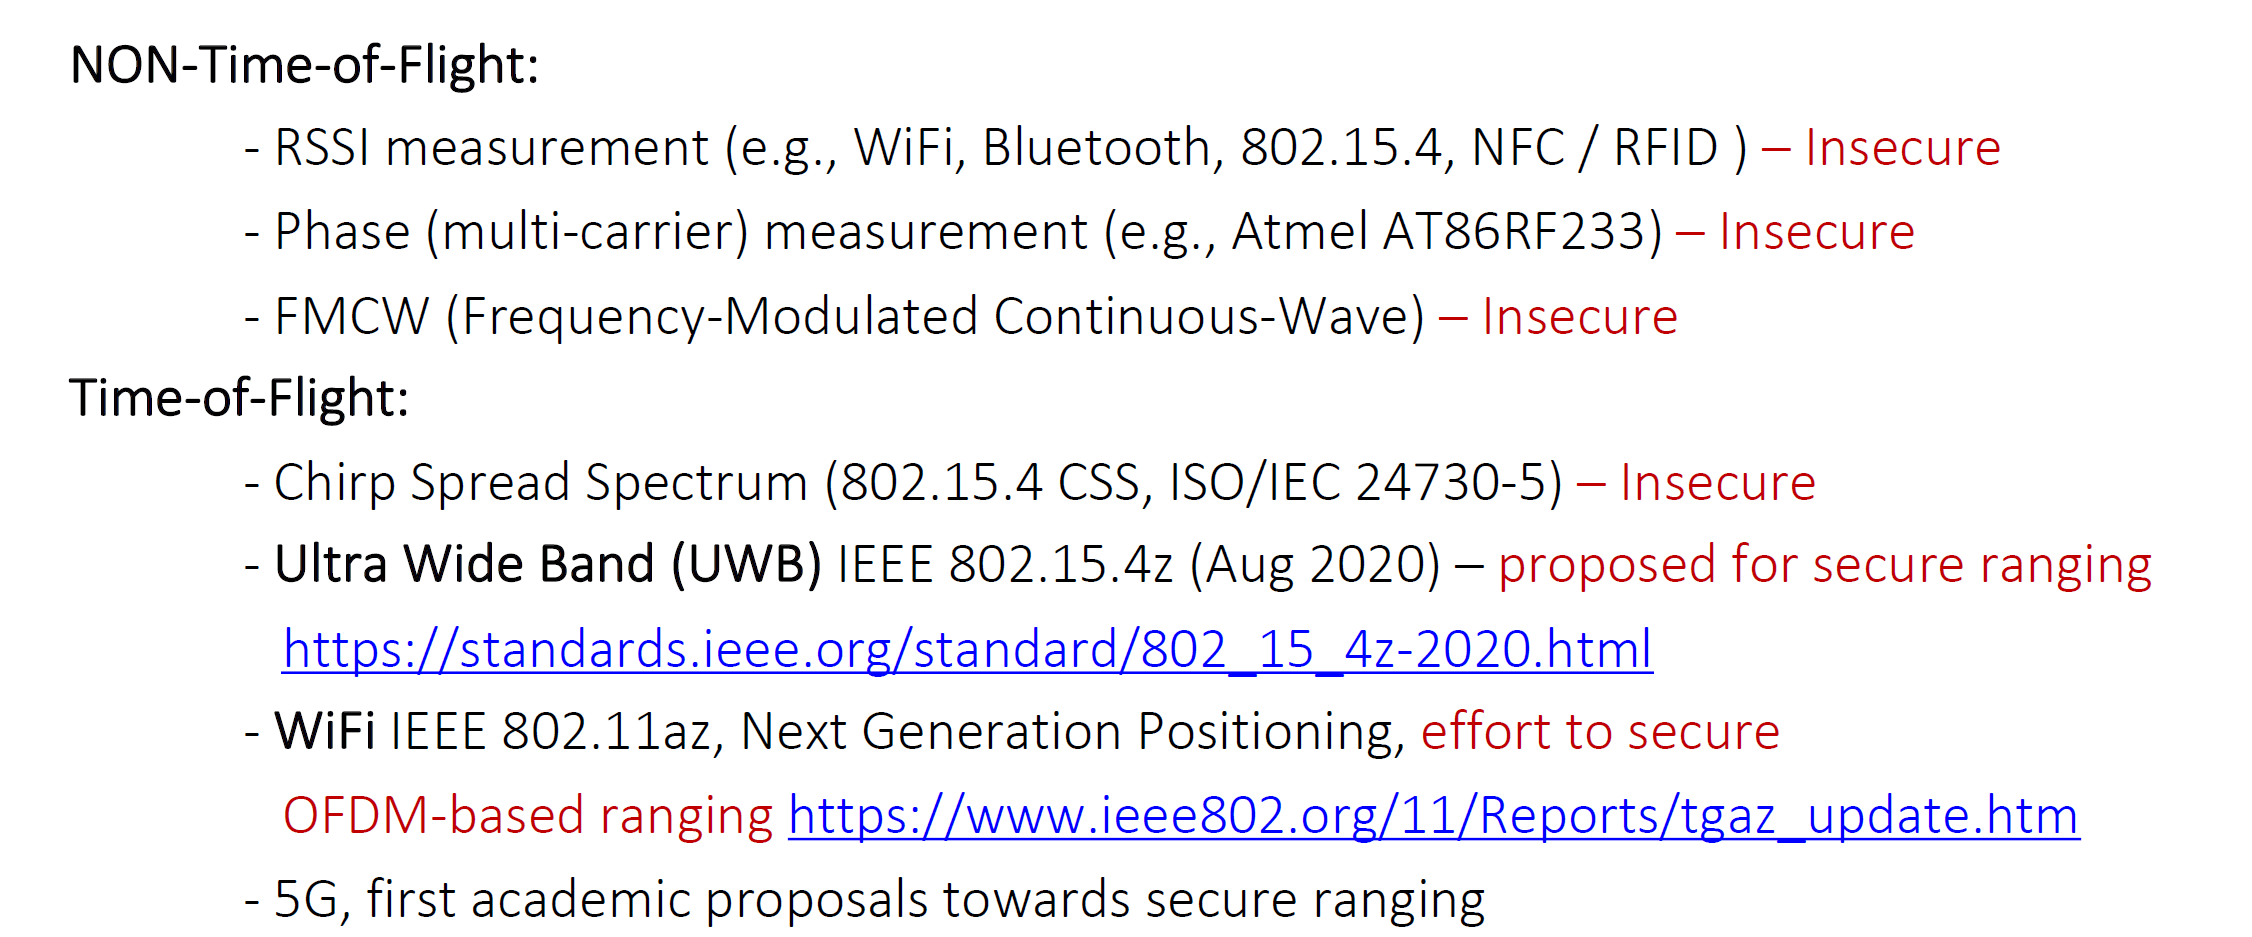
\includegraphics[width=\linewidth]{Figures/L5_ranging_techniques.PNG} 
\end{minipage}

\paragraph{Distance Bounding:} There are different scenarios and attacks. But the most common scenario is:\\
V and P want to measure distance and trust each other, M tries to manipulate this process.

\begin{minipage}{\linewidth}
    \centering      
    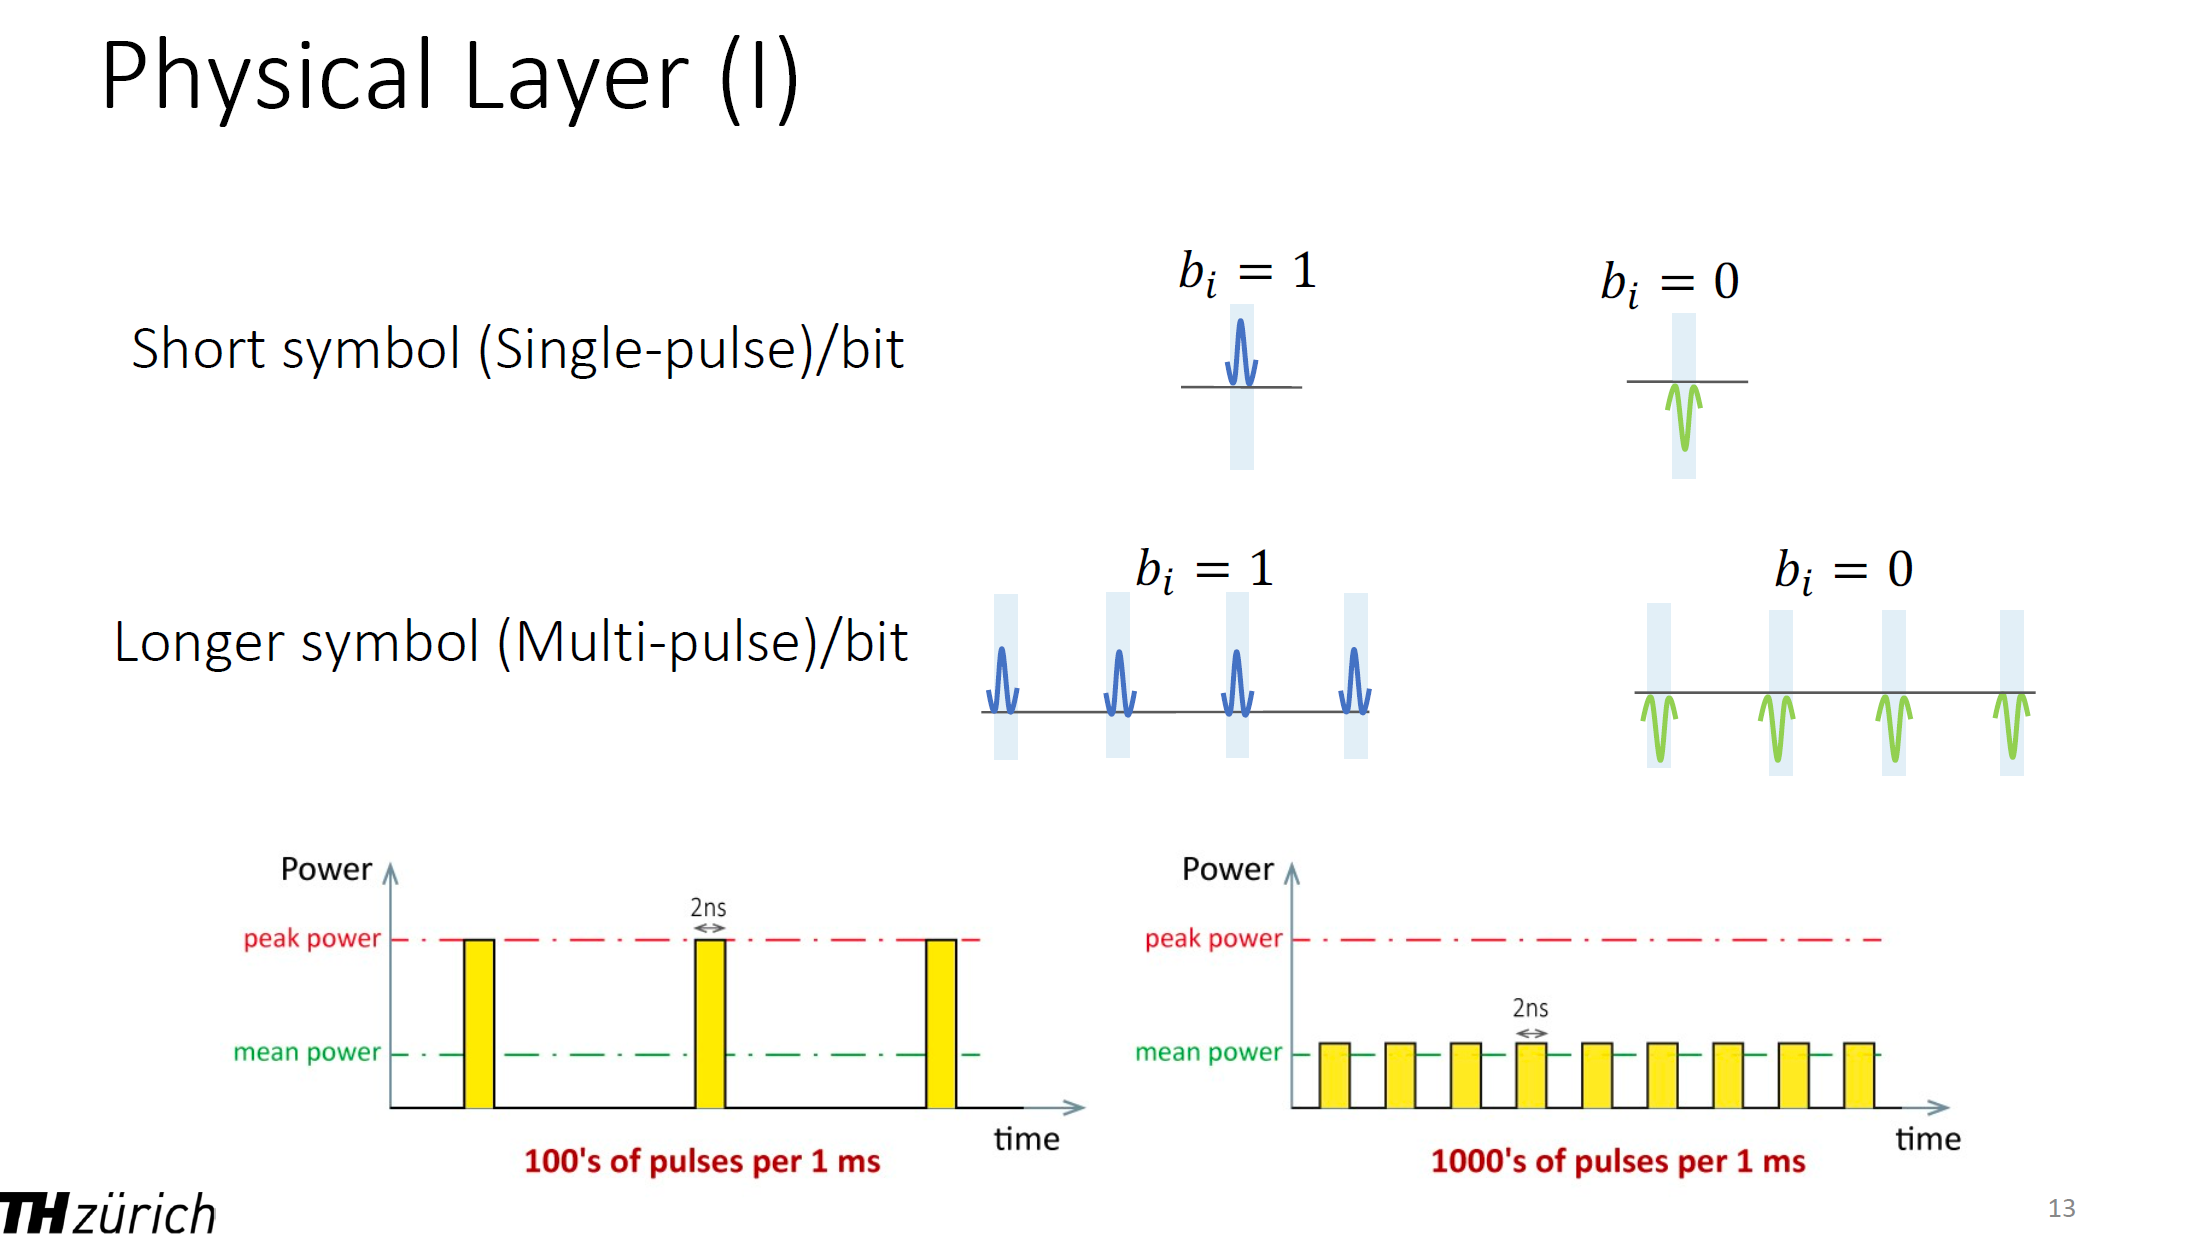
\includegraphics[width=\linewidth]{Figures/L5_physical_layer.PNG} 
\end{minipage}

\begin{minipage}{\linewidth}
    \centering      
    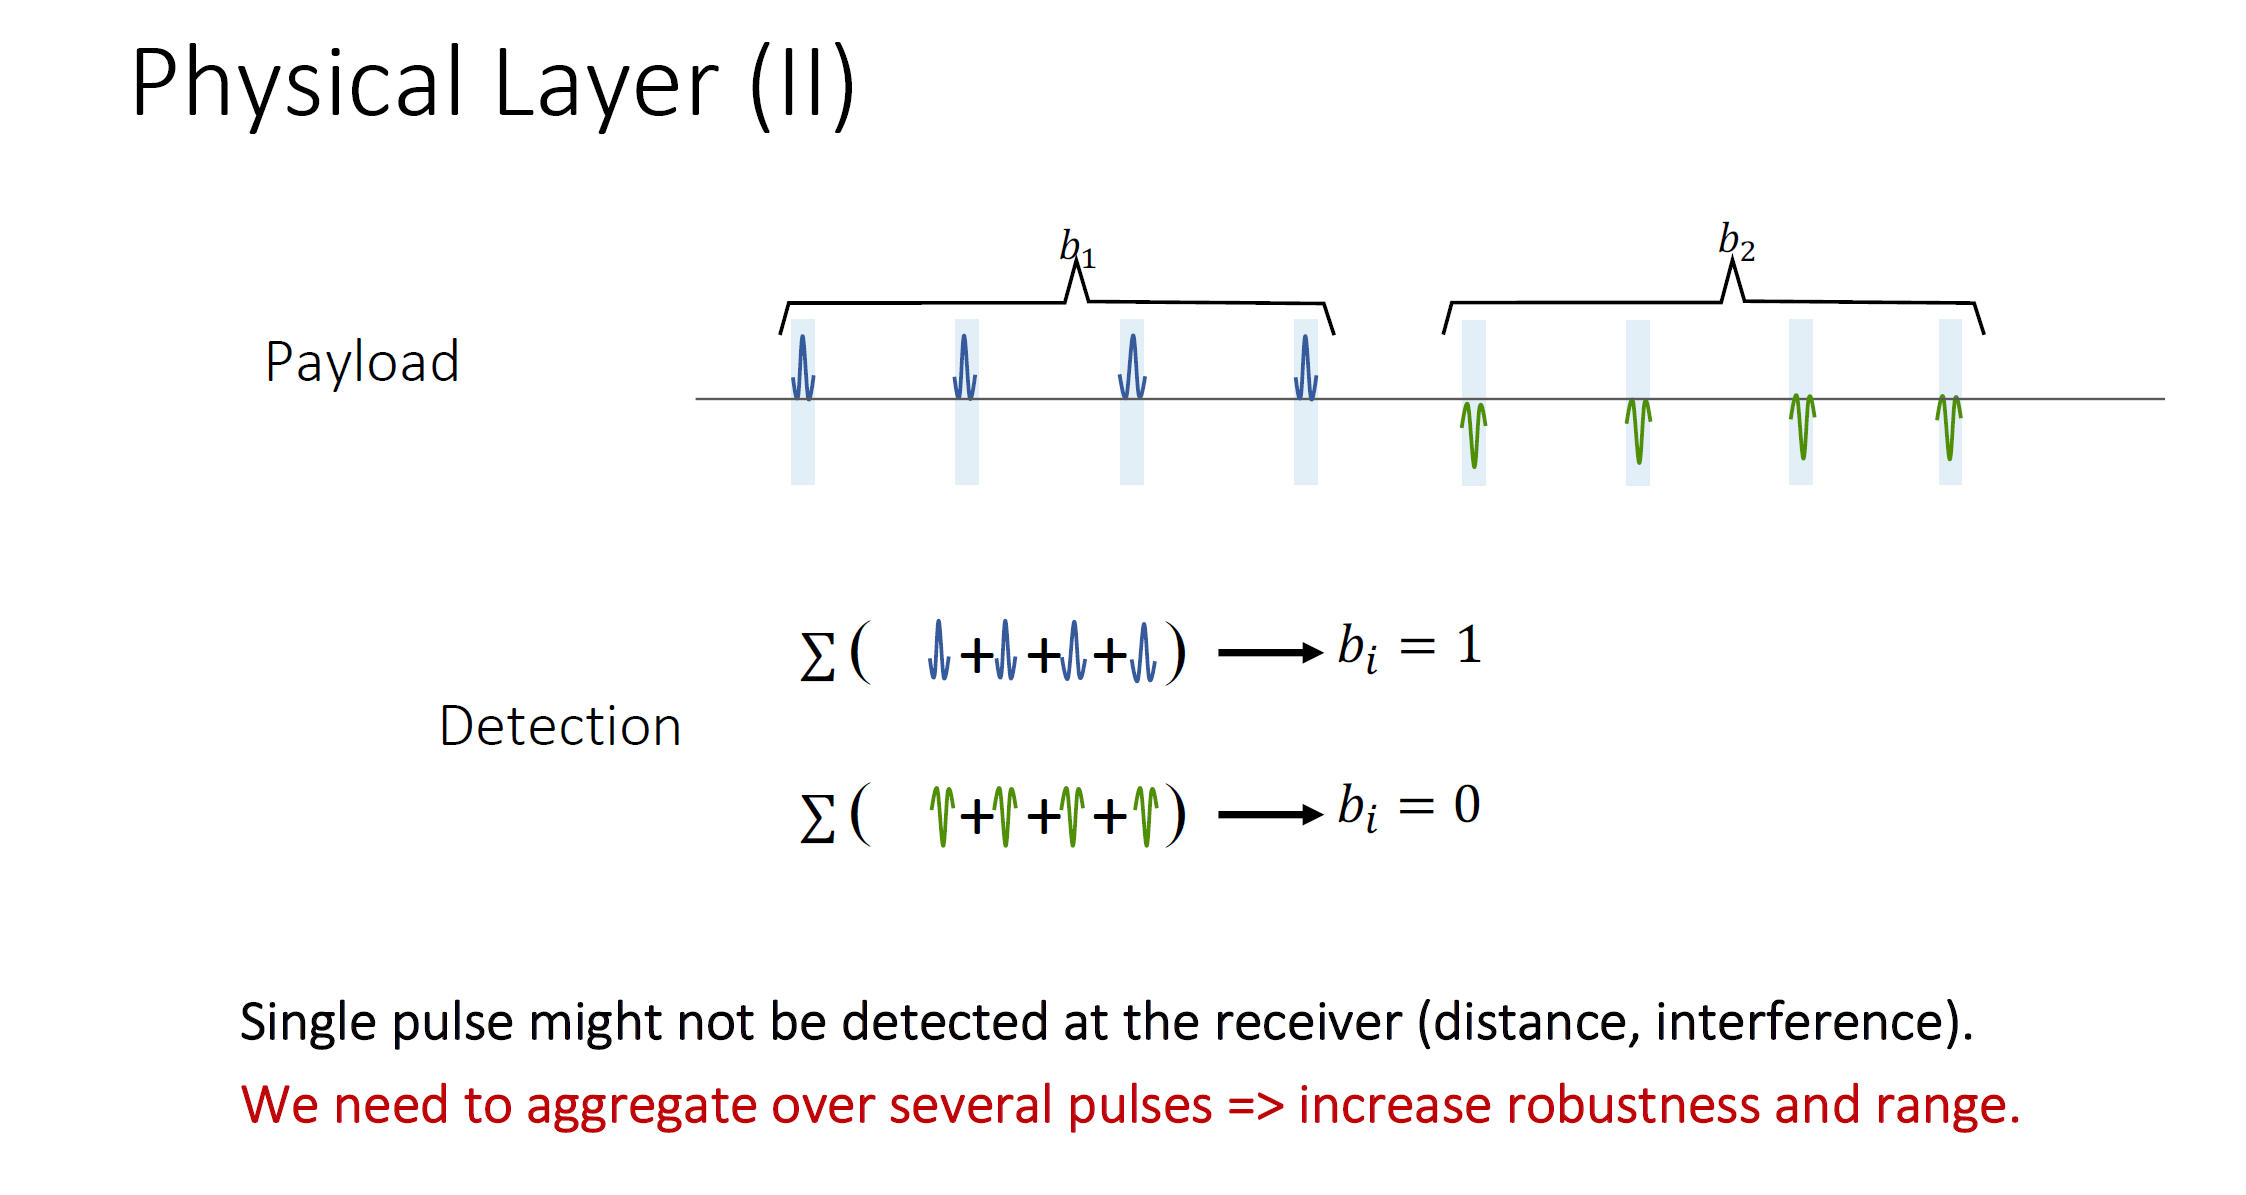
\includegraphics[width=\linewidth]{Figures/L5_physical_layer2.PNG} 
\end{minipage}

\begin{minipage}{\linewidth}
    \centering      
    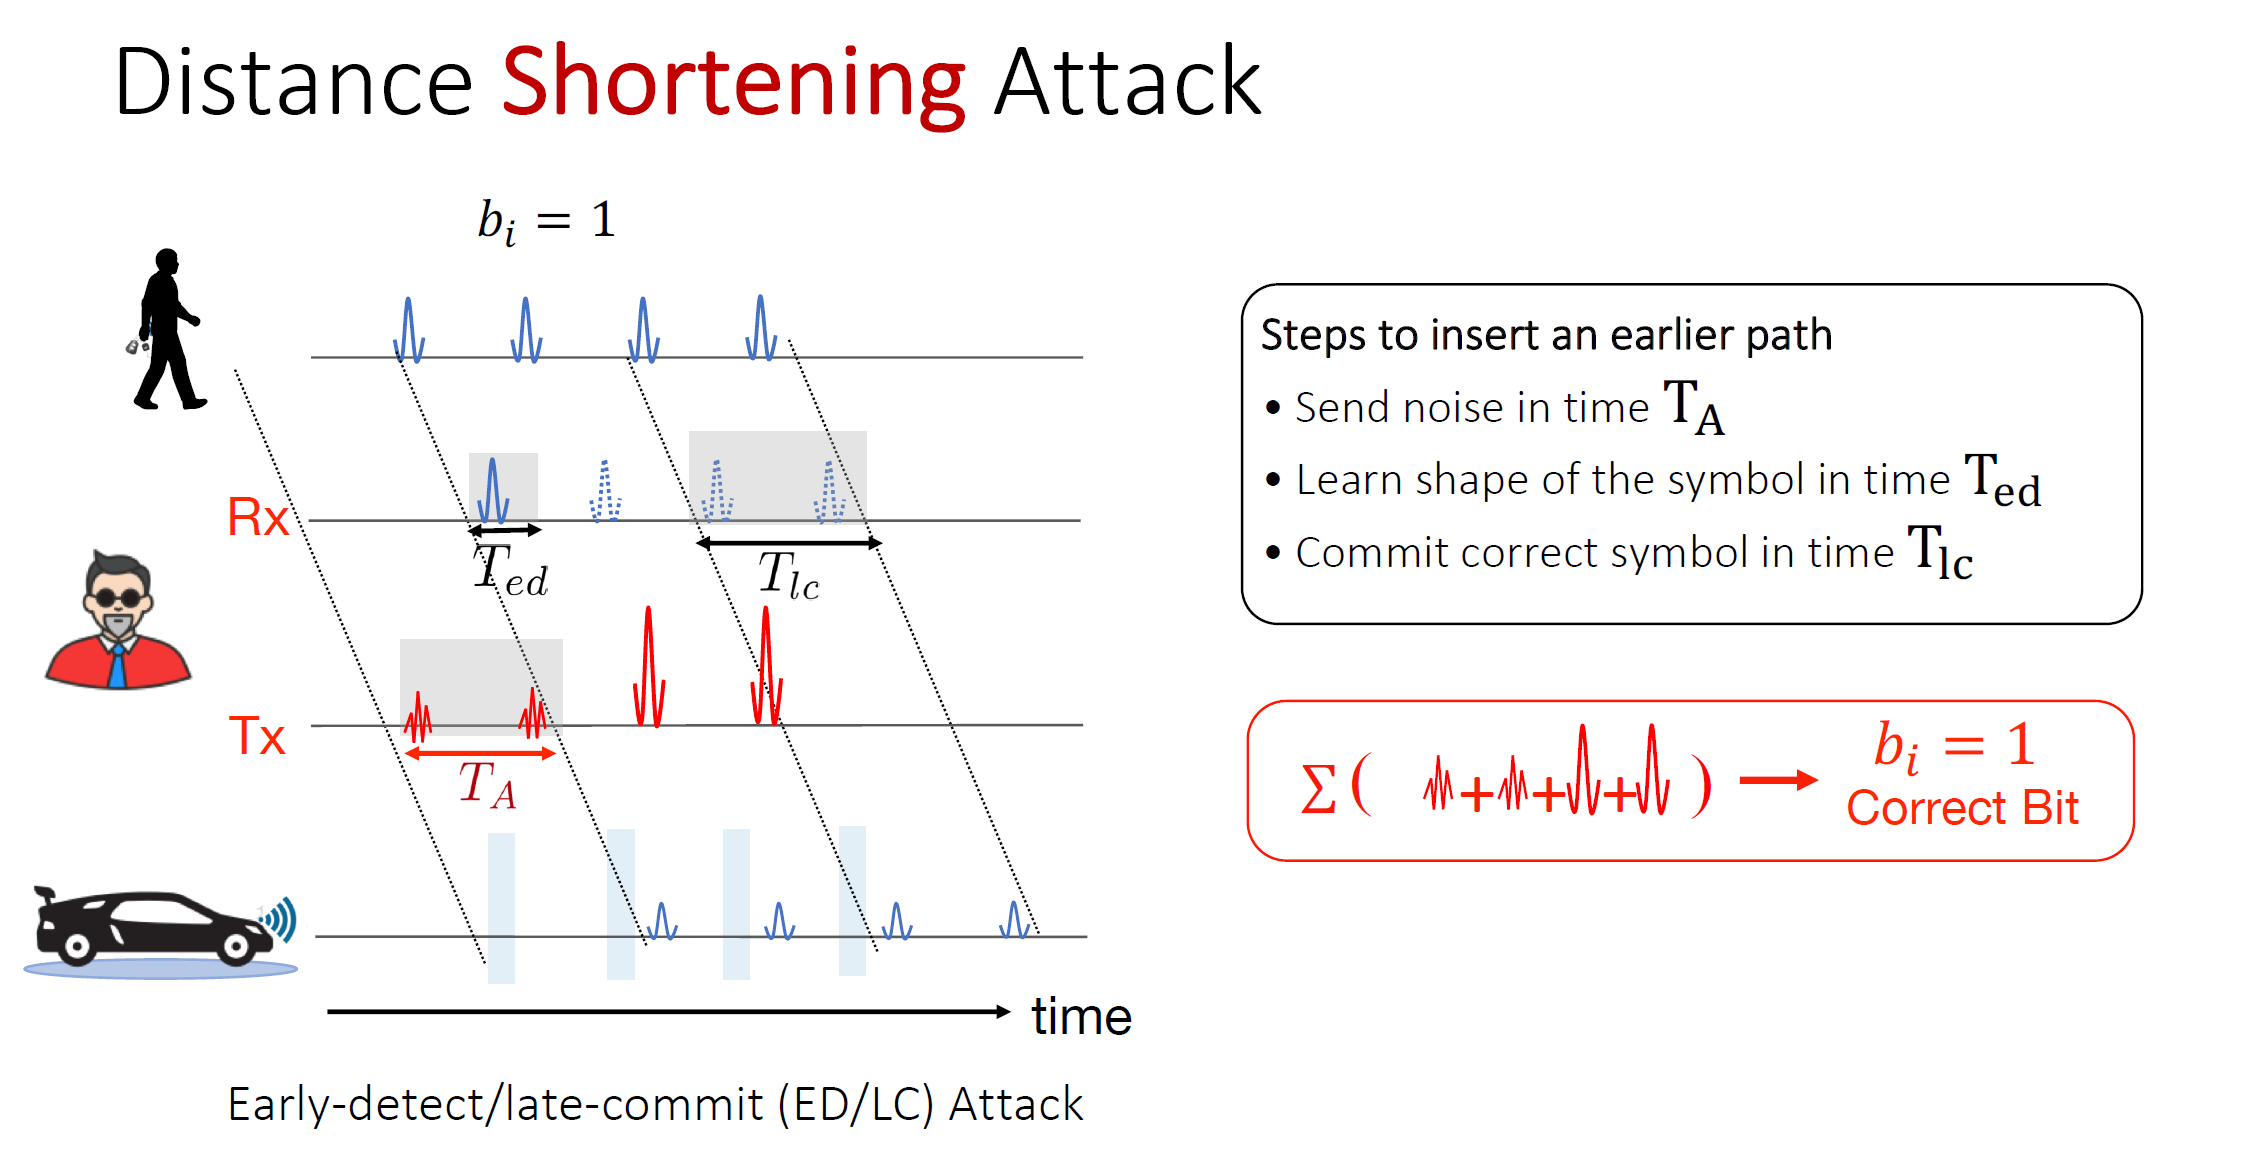
\includegraphics[width=\linewidth]{Figures/L5_shortening_attack.PNG} 
\end{minipage}

\paragraph{Performance/Security Tradeoff:} We need longer symbols (multi-pulse) for performance (range and robustness). However, longer symbols are vulnerable to above attack

\begin{minipage}{\linewidth}
    \centering      
    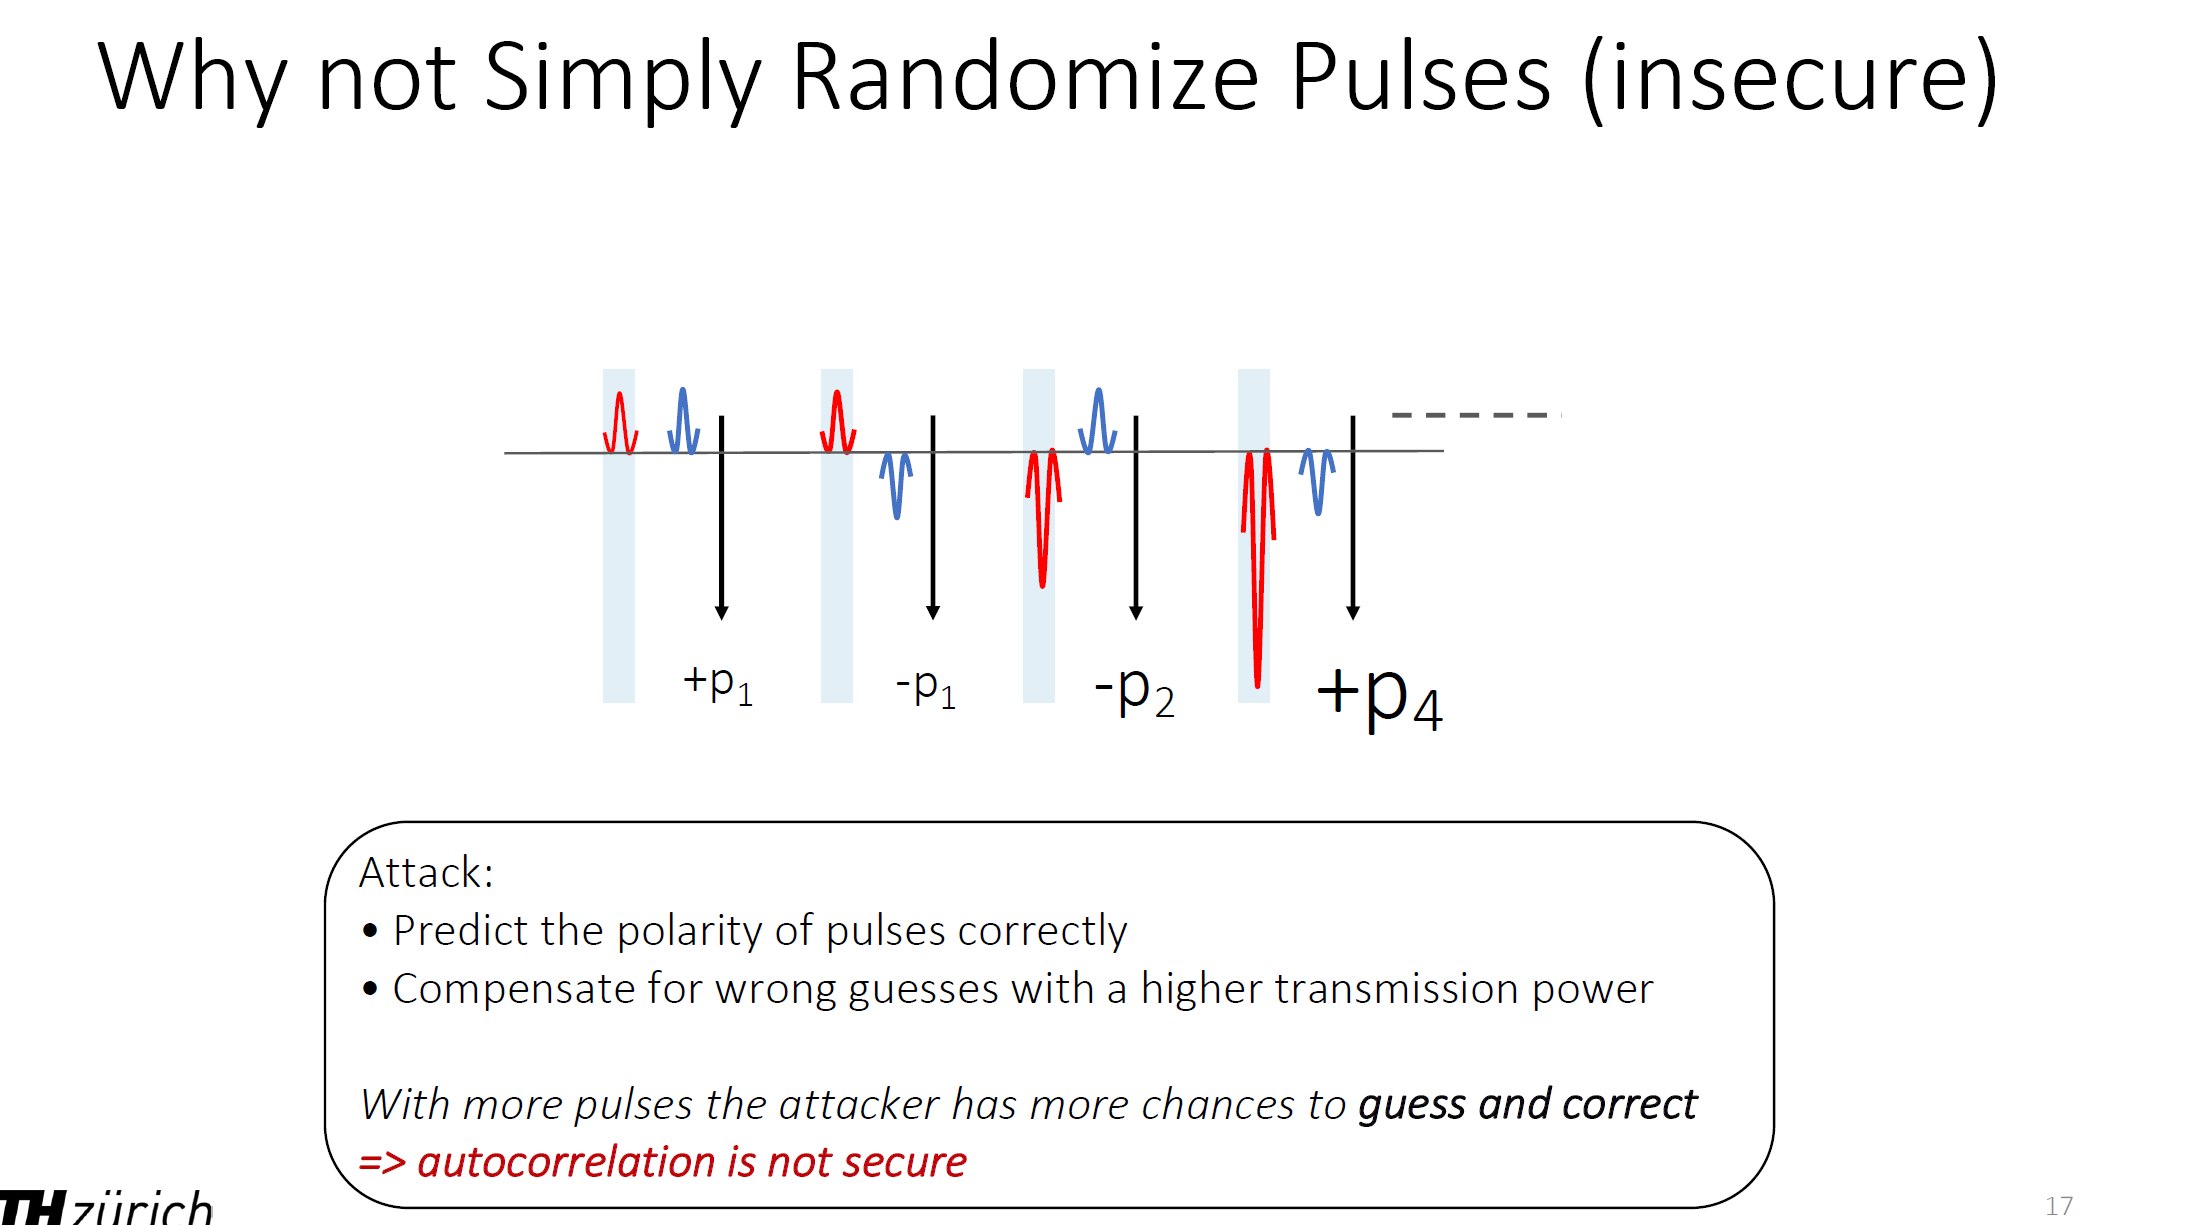
\includegraphics[width=\linewidth]{Figures/L5_pulse_randomization.PNG} 
\end{minipage}

\paragraph{Best case for Attacker and worst case for Users:}
\begin{itemize}
    \item Victims: Have to assume bad channel, noise, ...low SNR --> have to tolerat errors.
    \item Attacker: has perfect channel to the victim and no noise --> can guess and compensate (guesses will seem like noise and mpath)
\end{itemize}

\subsection{UWB Solutions}
\begin{minipage}{\linewidth}
    \centering      
    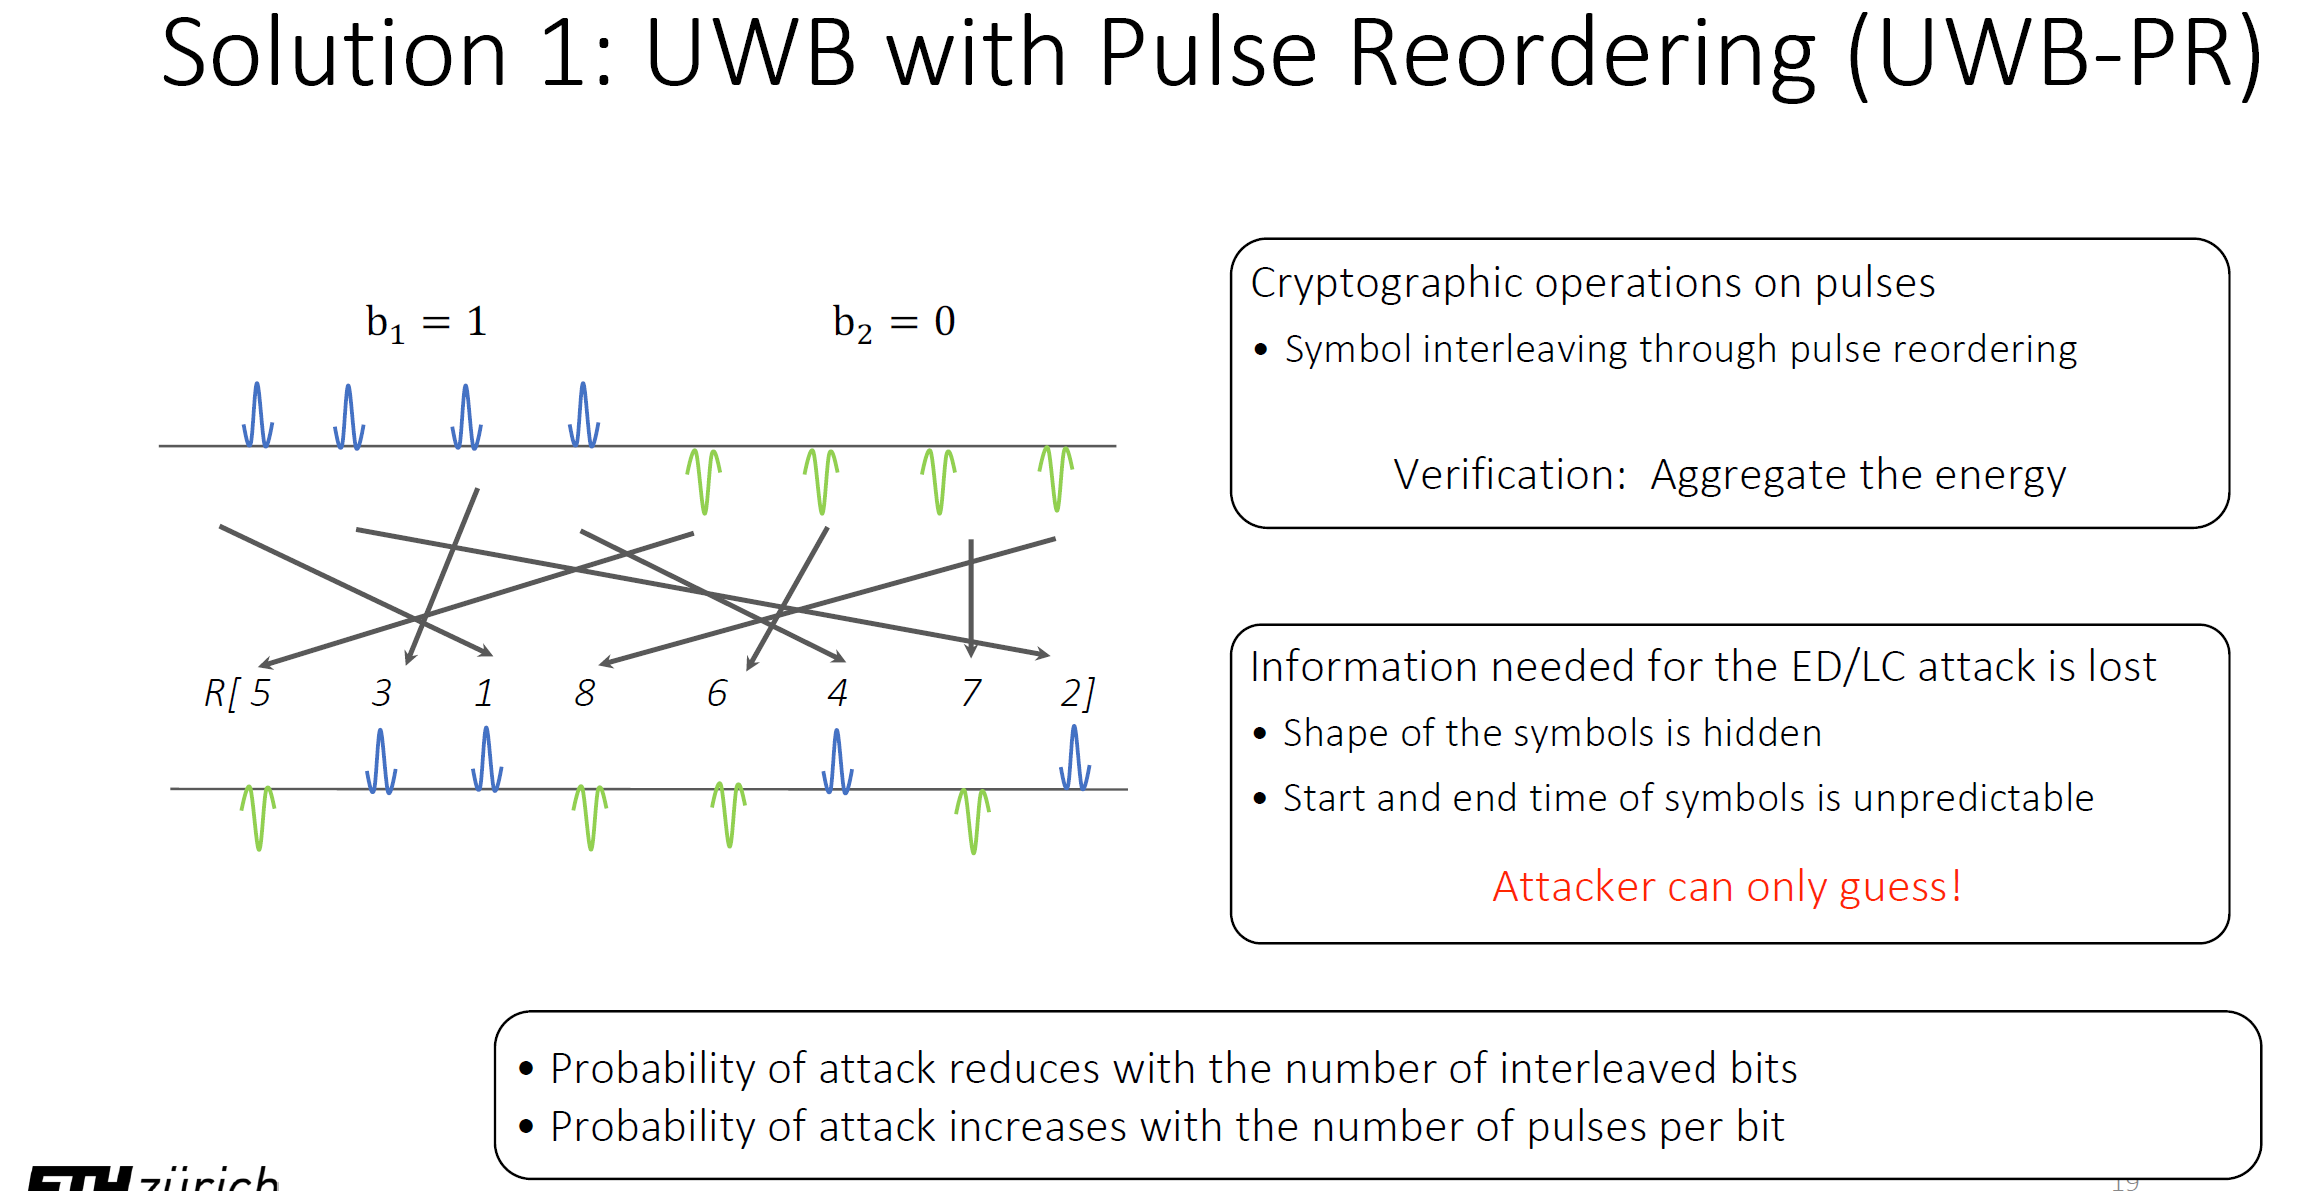
\includegraphics[width=\linewidth]{Figures/L5_sol1.PNG} 
\end{minipage}
\begin{minipage}{\linewidth}
    \centering      
    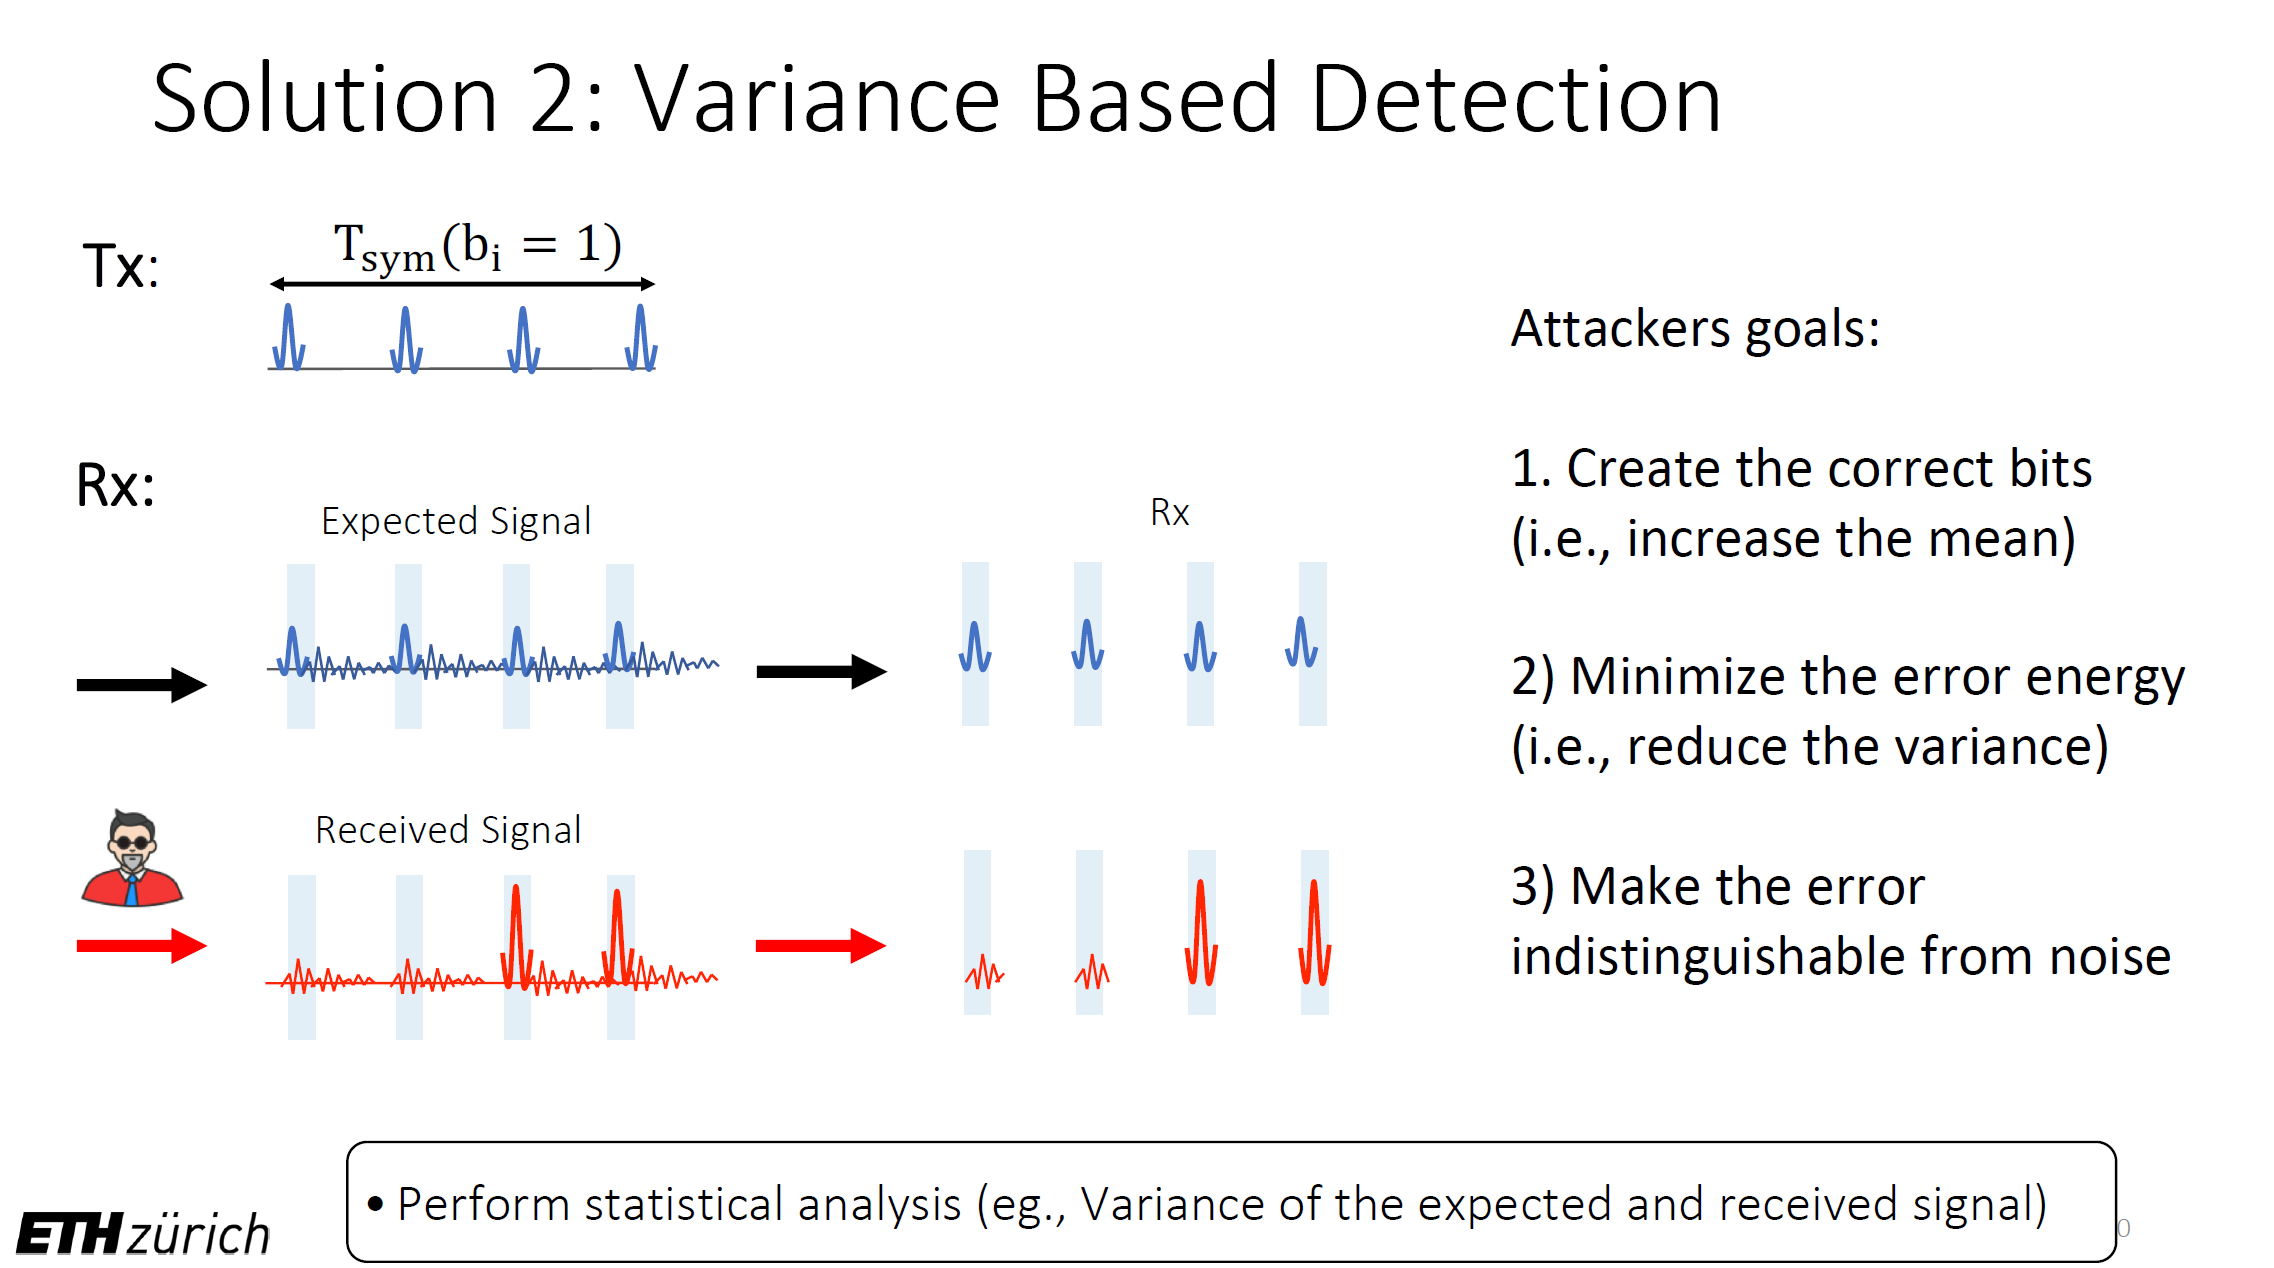
\includegraphics[width=\linewidth]{Figures/L5_sol2.PNG} 
\end{minipage}

\begin{minipage}{\linewidth}
    \centering      
    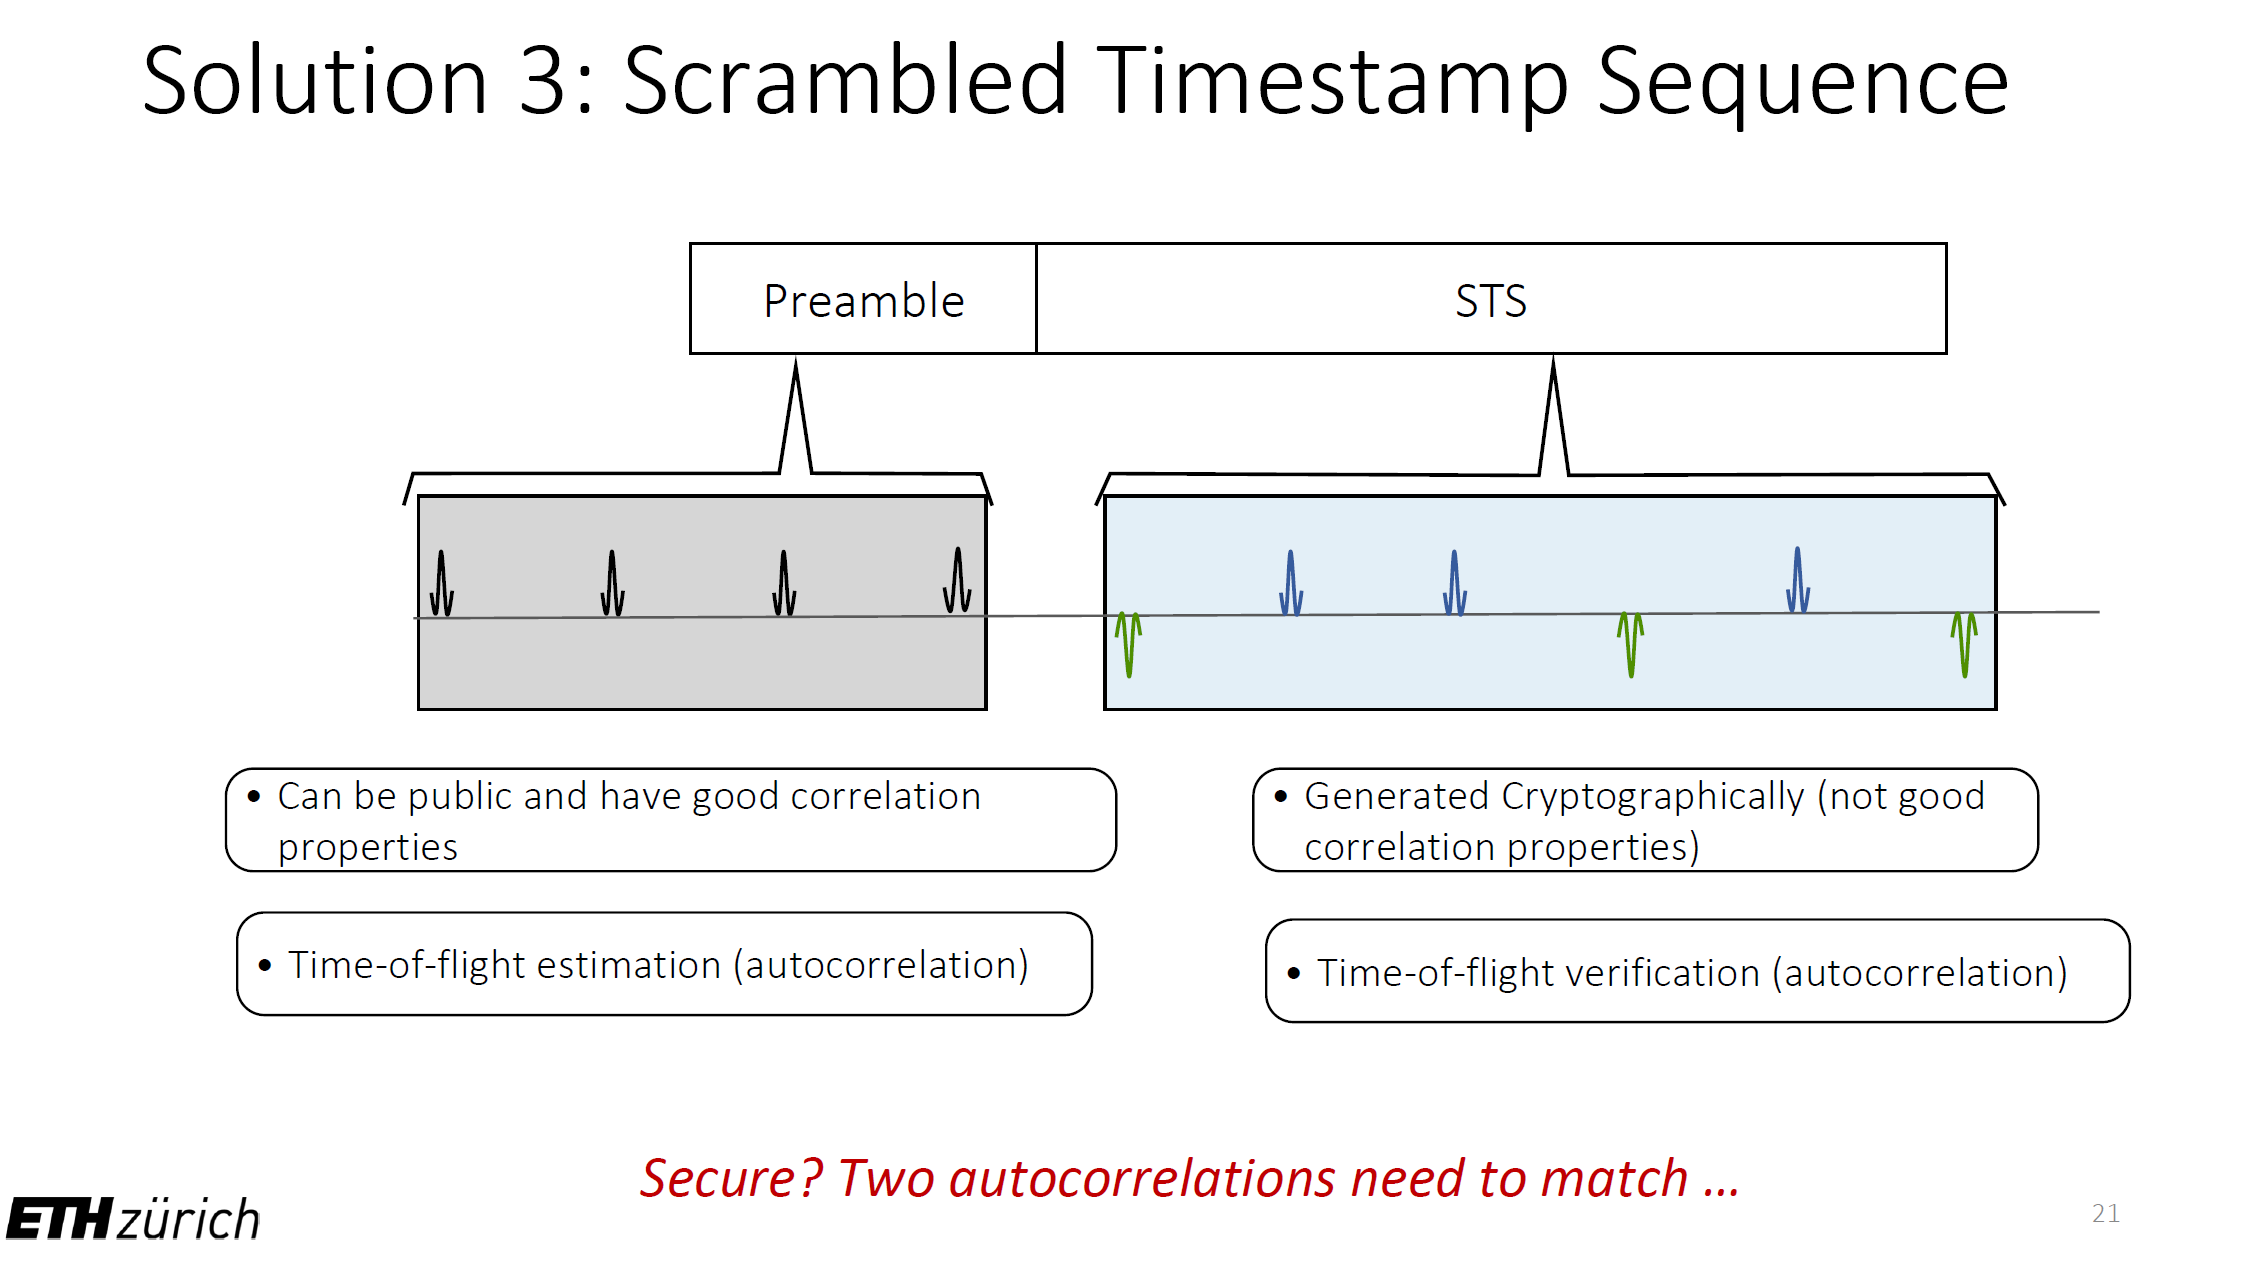
\includegraphics[width=\linewidth]{Figures/L5_sol3.PNG} 
\end{minipage}

\begin{minipage}{\linewidth}
    \centering      
    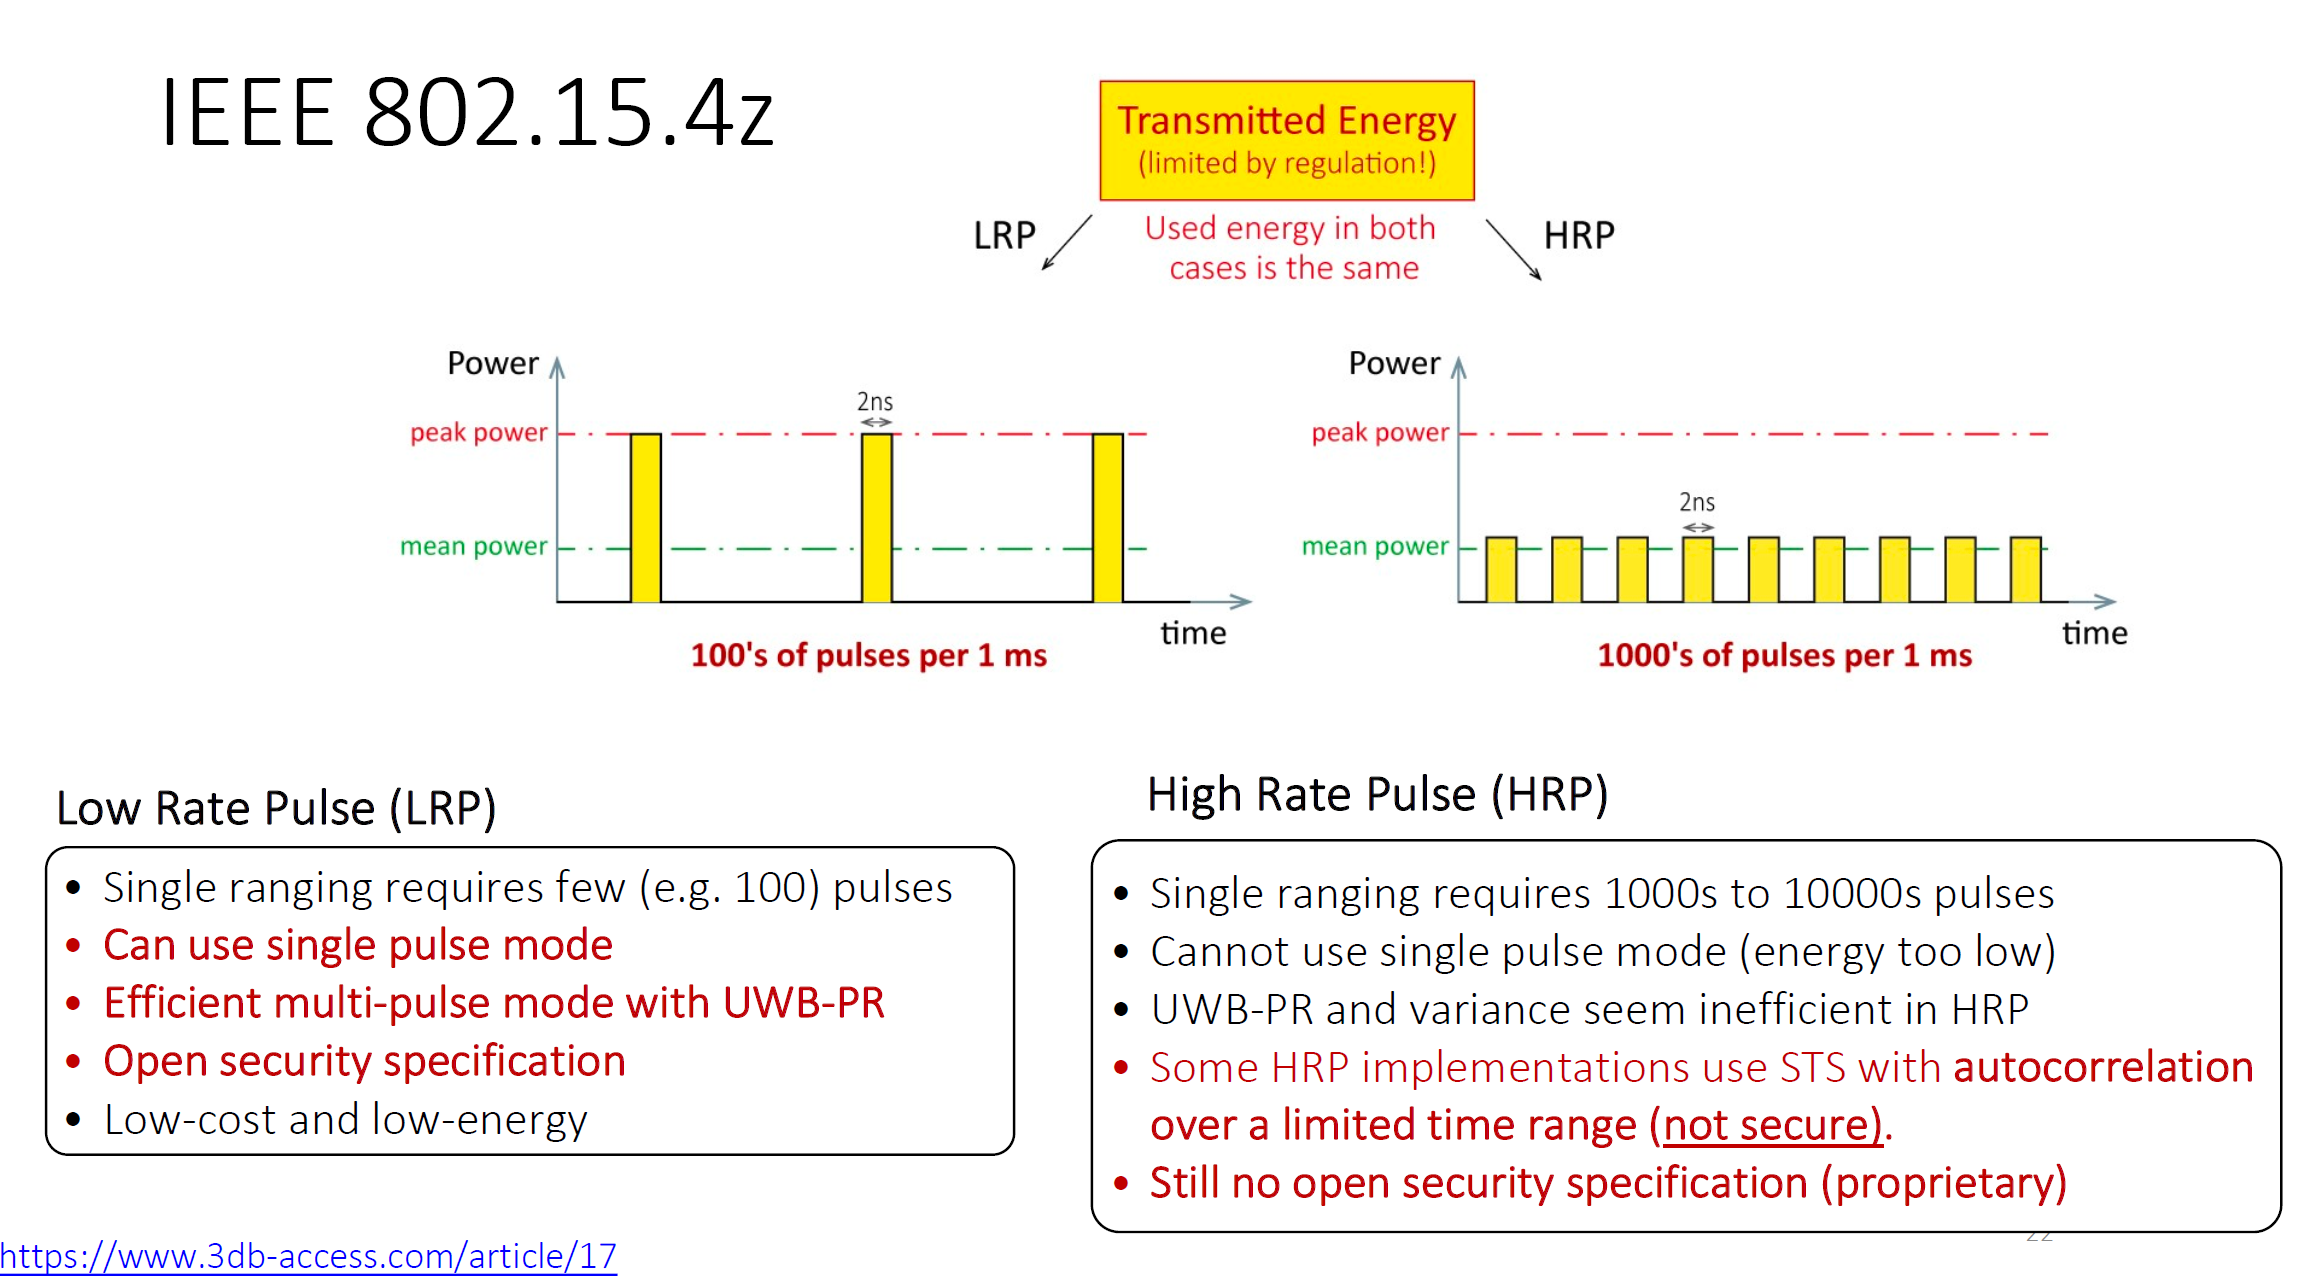
\includegraphics[width=\linewidth]{Figures/L5_IEEE.PNG} 
\end{minipage}

\begin{minipage}{\linewidth}
    \centering      
    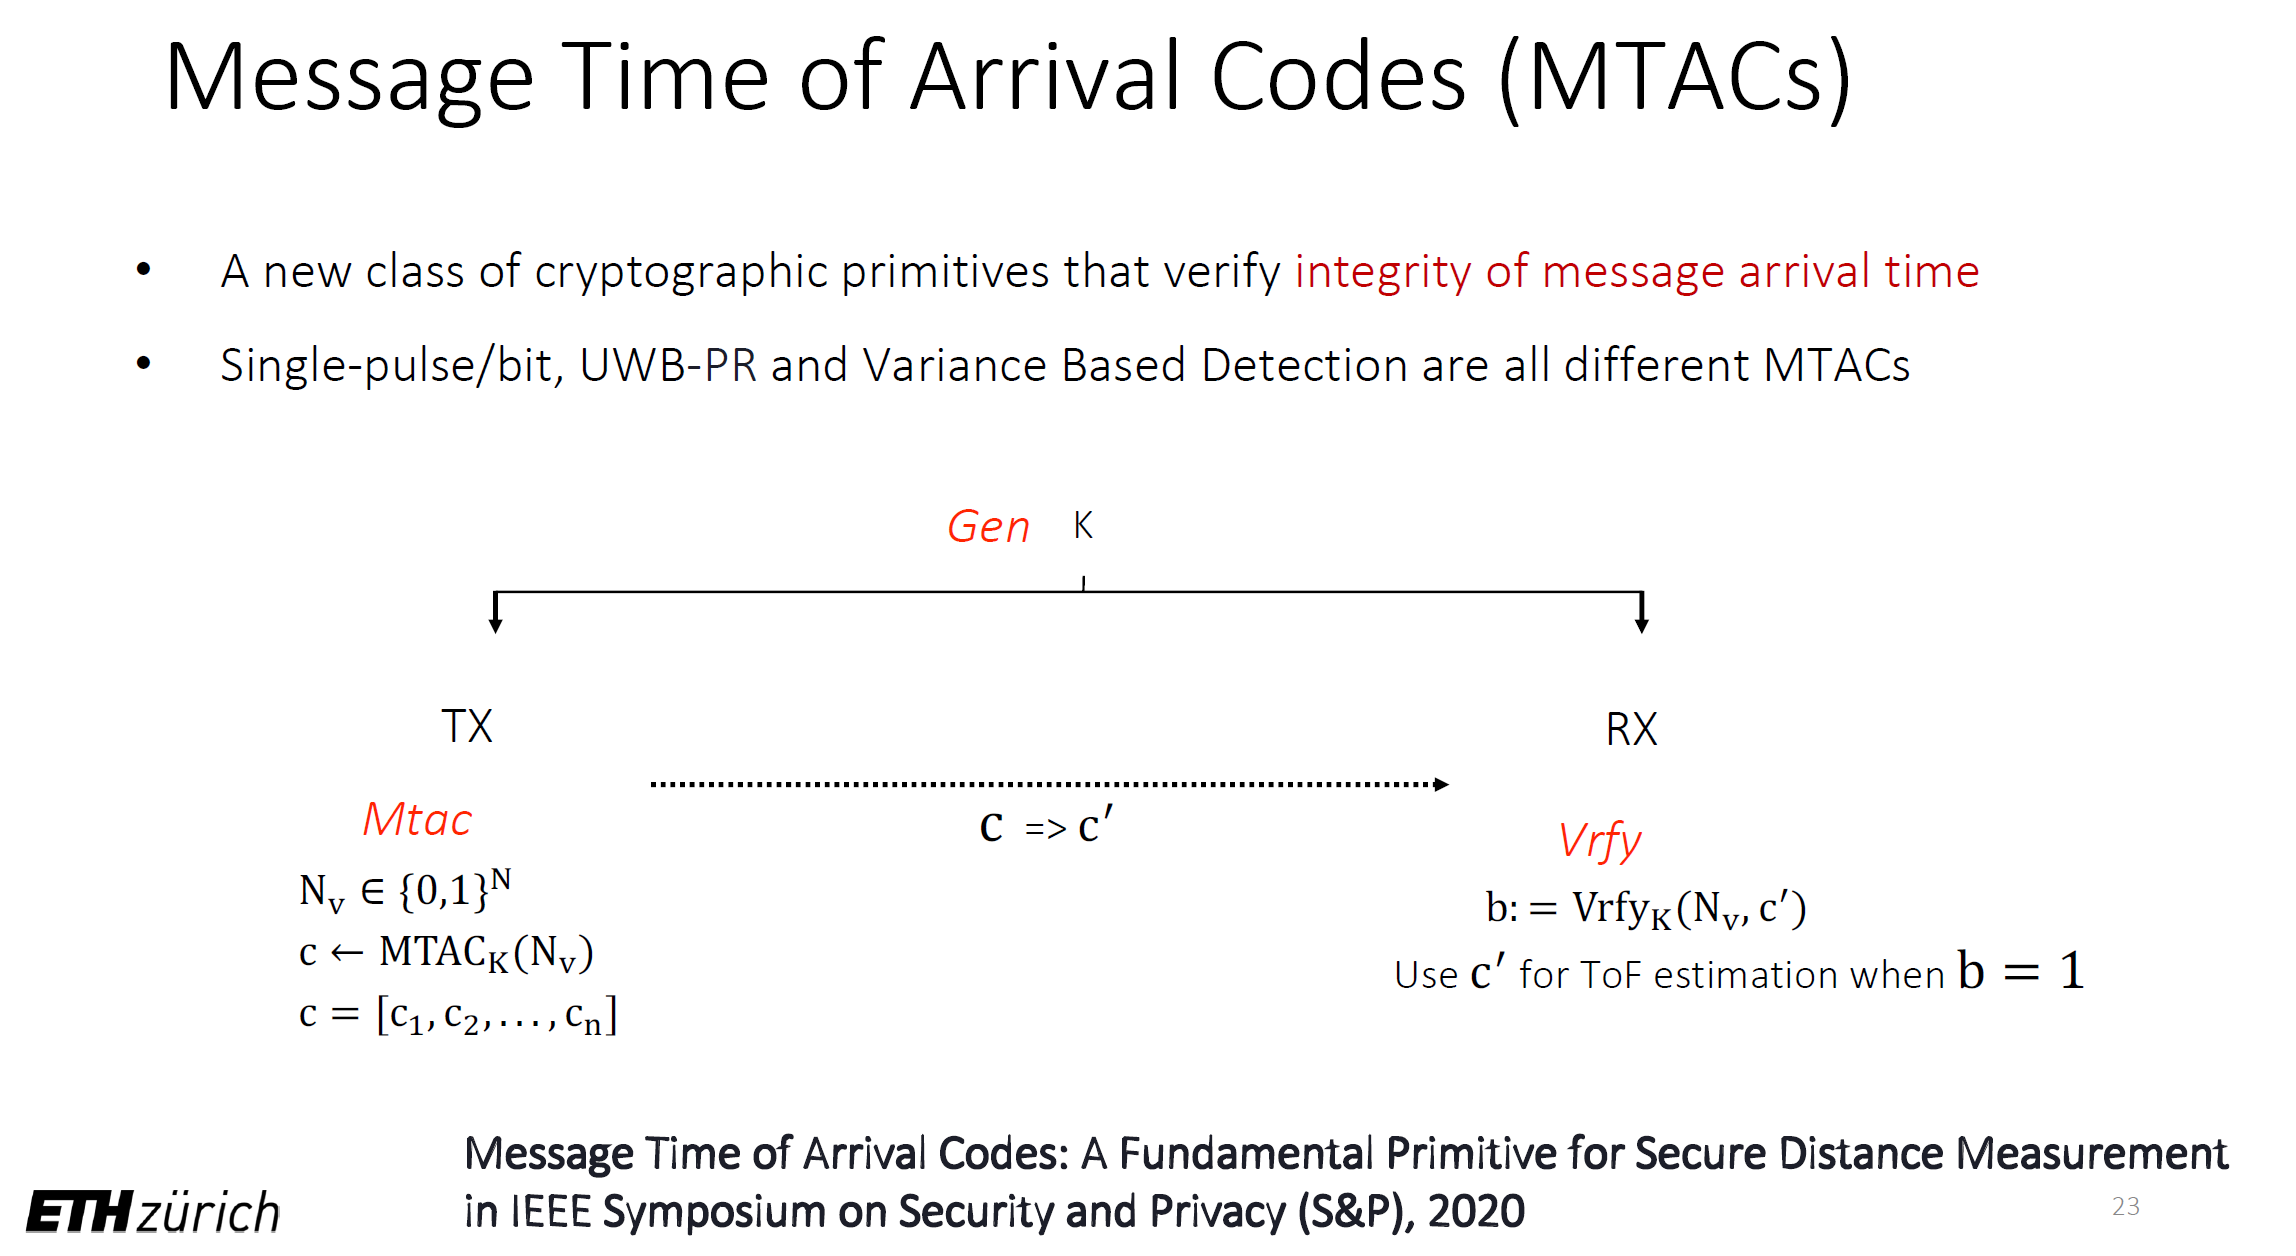
\includegraphics[width=\linewidth]{Figures/L5_MTAC.PNG} 
\end{minipage}

\paragraph{UWB Summary:} 
\begin{itemize}
    \item UWB can be used to provide precise, performant, and secure ranging
    \begin{itemize}
        \item Can use challenge-response protocol at logical layer.
        \item Distance commitment at the physical layer
        \item Design MTACs (Gen,Mtac,Vrfy) to preserve the integrity of arrival time.
    \end{itemize}
    \item 80.15.4z: 
    \begin{itemize}
        \item LRP open and secure in both single-pulse/bit and multi-pulse/bit modes
        \item HRP security is proprietary and needs further analysis.
        \item Attacks exist on different HRP implementations
        \item Not clear if we can build a fully secure and efficient HRP based system.
    \end{itemize}
\end{itemize}

\subsection{Secure Ranging in 5G}
TODO